\section{Results}\label{sec:results}
\subsection{Radiation-era stability}
The scalar radiation-sector characteristic polynomial is
\begin{equation}
A\lambda^2+B\lambda+C=0,
\end{equation}
with
\begin{align}
A&=\frac{2I_0K_B}{\Q a^3}-4K_B+8,\\
B&=HA,\\
C&=\frac{2HI_0(2-K_B)}{a^3}.
\end{align}
On the expanding physical branch $H>0$, $I_0>0$, $\Q>0$, $a>0$, and $0<K_B<2$, all three coefficients are positive. The quadratic is therefore strictly Hurwitz. Removing the nonseparable mixed-current operator recovers the slow/zero-mode defect, establishing that strict damping is a consequence of the nonseparable structure rather than of the unchanged FLRW background.

The corresponding high-frequency scalar sound speed is
\begin{equation}
c_s^2=\frac{4K_2K_BZ_0\sinh[(\Q-\Q_0)/Z_0]/\Q+4(2-K_B)}{4K_2K_B\cosh[(\Q-\Q_0)/Z_0]},
\label{eq:cs2}
\end{equation}
which remains positive on the tested branch. Internal radiation histories were finite and bounded, the expected horizon crossings were observed, CMB spectra remained finite through $\ell=2500$, and $P(k)$ remained finite and positive over the publication regression range.

\begin{figure}[htbp]
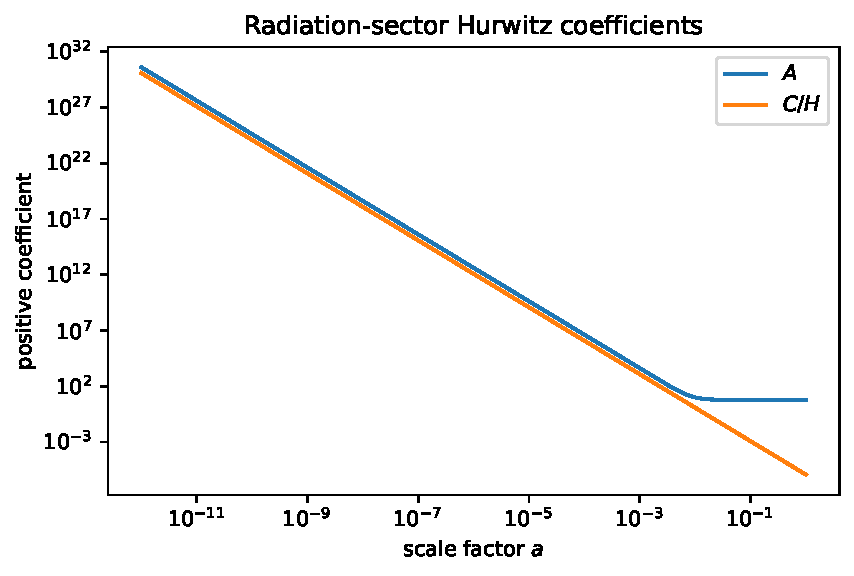
\includegraphics[width=\columnwidth]{figures/fig_radiation_stability.pdf}
\caption{Positive coefficients controlling the scalar radiation-sector Hurwitz polynomial along the tested background.}
\label{fig:hurwitz}
\end{figure}

\subsection{Matched operator-removal response}
At fixed homogeneous parameters and initial conditions, removing the mixed-current contribution produces a nonzero perturbative response. The maximum normalized differences are $0.3269$ internally, $0.3269$ in $E$, $0.2018$ in $\chi$, $7.11\times10^{-4}$ in $\delta$, and $9.87\times10^{-4}$ in $\theta$. The maximum relative differences in the tested CMB and linear matter spectra are $7.01\times10^{-3}$ and $2.18\times10^{-1}$, respectively. These values demonstrate that the operator has a causal perturbation-level role while leaving the homogeneous expansion unchanged.

\begin{figure}[htbp]
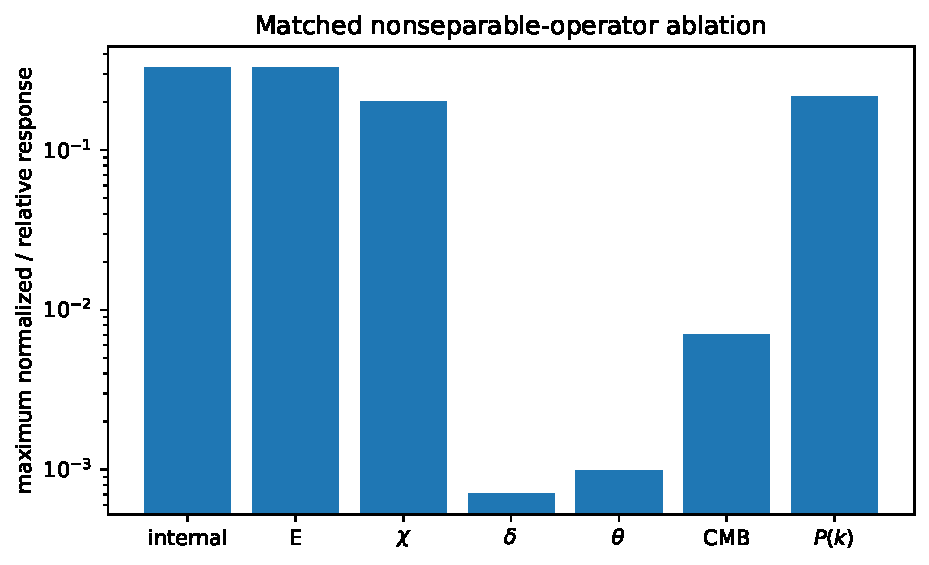
\includegraphics[width=\columnwidth]{figures/fig_operator_ablation.pdf}
\caption{Matched operator-removal response. The homogeneous background, initial conditions, and numerical settings are fixed while the nonseparable direct scalar contribution is removed in the control calculation.}
\label{fig:ablation}
\end{figure}

\subsection{Degrees of freedom and effective-field-theory scale}
The analyzed nonlinear phase space has dimension 42, with six first-class and eighteen second-class constraints, giving
\begin{equation}
N_{\rm dof}=\frac{42-2(6)-18}{2}=6.
\end{equation}
The auxiliary acceleration sector introduces no additional propagating scalar after its constraints are eliminated, while the nonseparable scalar operator changes neither the number of configuration variables nor the highest time-derivative order.

Including the temporal, mixed, and MOND cubic vertices, the canonically normalized propagating scalar has
\begin{equation}
\Lambda_{\rm sc,min}=1.47423693\times10^{-6}\ {\rm eV}
\end{equation}
at $a=6.44196\times10^{-3}$, where the mixed vertex controls the minimum. The minimum ratio of this scale to the tested reference expansion scale exceeds $1.7\times10^{10}$.

The companion scalar is first order. After solving its second-class constraints,
\begin{equation}
\Theta_{\rm red}=p_\chi d\chi-\Delta_k\Phi\,du,
\end{equation}
with
\begin{equation}
\Delta_k=ak^2+\frac32I_0\Q
\end{equation}
in the conservative matter-free case and an additional positive $\frac32a^3\rho_m$ term with matter. The tested minimum is $6.0136920\times10^{-8}\,\mathrm{Mpc}^{-2}$ and $\Delta_k^{-1}\sim k^{-2}$ at high $k$, so the constraint reduction is infrared finite and ultraviolet soft.

\subsection{Final cosmological likelihood}
Table~\ref{tab:likes} gives the independently replayed likelihood contributions. Their sum is
\begin{equation}
\chi^2_{\rm MG}=2422.695966726233.
\end{equation}
The matched optimized $\LCDM$ reference has $\chi^2=2428.9192$, so
\begin{equation}
\Delta\chi^2_{\rm MG-\LCDM}=-6.2232333.
\end{equation}
For seven fitted coordinates in the modified-gravity realization and six in the reference model, using the matched-analysis convention $N=2392$ for BIC,
\begin{align}
\Delta\mathrm{AIC}_{\rm MG-\LCDM}&=-4.2232333,\\
\Delta\mathrm{BIC}_{\rm MG-\LCDM}&=+1.5566518.
\end{align}
Thus the maximum likelihood and AIC favor the modified-gravity realization in this matched comparison, whereas BIC gives a small preference to the lower-dimensional $\LCDM$ reference. Because the models are not being treated here as a one-parameter nested hypothesis test, we do not assign a Gaussian significance by taking $\sqrt{|\Delta\chi^2|}$.

\begin{table}[htbp]
\caption{Independent fresh likelihood evaluation at the final optimized point.}\label{tab:likes}
\begin{ruledtabular}
\begin{tabular}{lr}
Likelihood & $\chi^2$\\\hline
Planck high-$\ell$ TTTEEE-lite & 582.162661\\
Planck low-$\ell$ TT & 22.975009\\
Planck low-$\ell$ EE & 395.918446\\
Planck lensing & 8.967854\\
DESI DR2 BAO & 8.640020\\
Pantheon+ & 1404.031978\\\hline
Total & 2422.695967\\
\end{tabular}
\end{ruledtabular}
\end{table}

\begin{figure}[htbp]
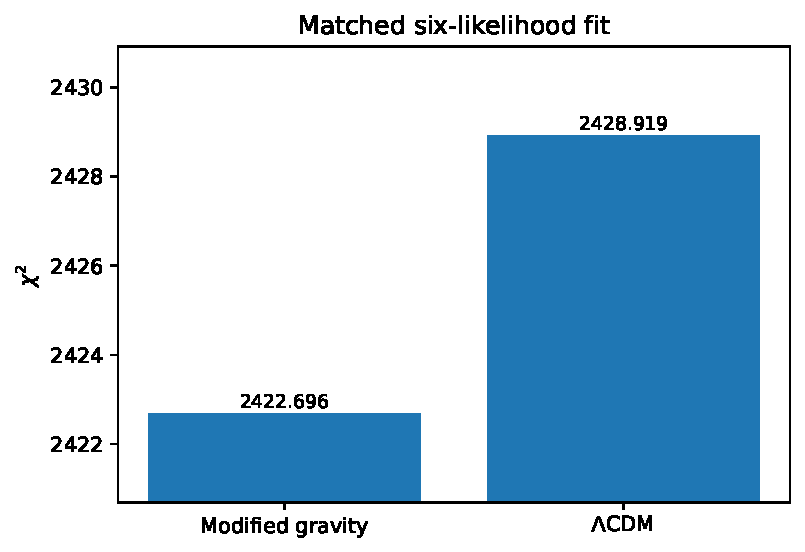
\includegraphics[width=\columnwidth]{figures/fig_chi2_comparison.pdf}
\caption{Total six-likelihood $\chi^2$ for the final modified-gravity realization and the matched optimized $\LCDM$ reference.}
\label{fig:chi2}
\end{figure}

\begin{figure}[htbp]
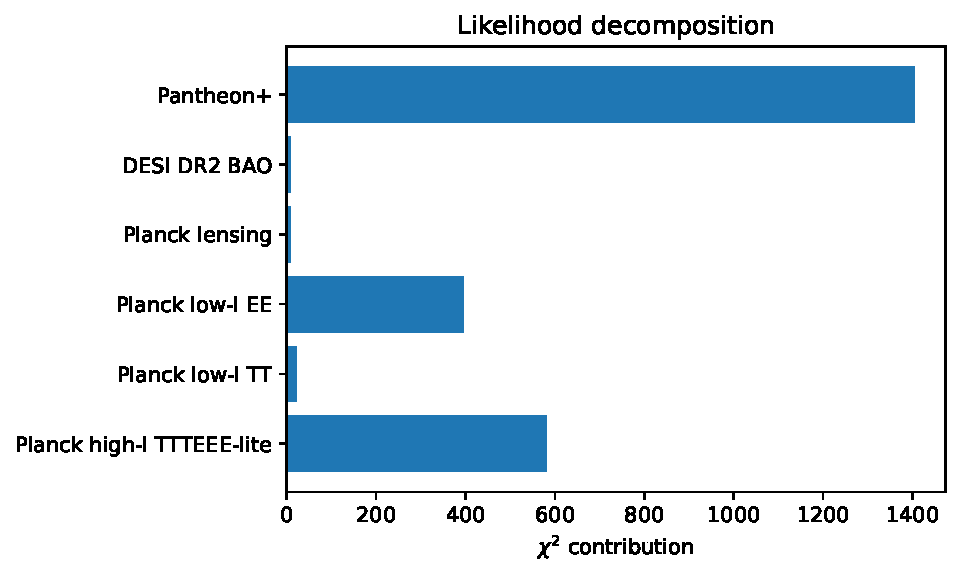
\includegraphics[width=\columnwidth]{figures/fig_likelihood_components.pdf}
\caption{Individual contributions to the final modified-gravity likelihood total.}
\label{fig:components}
\end{figure}

\subsection{Particle-CDM profile}
The independent profile has its lowest sampled value at $\omega_{\rm cdm}=0.001$. The exact zero-CDM point lies only
\begin{equation}
\Delta\chi^2(\omega_{\rm cdm}=0)=0.9581186
\end{equation}
above that sampled minimum. Thus the zero-particle-CDM realization is within $\Delta\chi^2<1$ of the profiled minimum. Across the tested grid the effective AeST cold density readjusts as explicit particle CDM is introduced. The appropriate conclusion is therefore that these data do not require nonzero particle CDM; they do not uniquely select exactly zero particle CDM.

\begin{figure}[htbp]
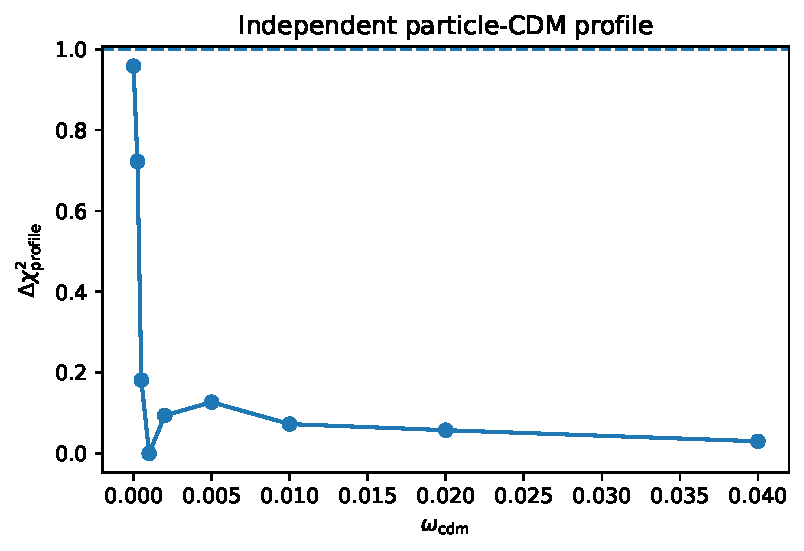
\includegraphics[width=\columnwidth]{figures/fig_cdm_profile.pdf}
\caption{Independent particle-CDM profile after reoptimization of the effective cold and cosmological coordinates at each sampled $\omega_{\rm cdm}$.}
\label{fig:profile}
\end{figure}

\subsection{Static galactic test}
In the screened static configuration $\Q=\Q_0$, so $\Gamma(\Q_0)=0$. The same $J(\Y)$ function therefore governs the static galaxy calculation. On the retained 132-galaxy, 2654-point SPARC subset, the baryons-only RMS scatter is $0.5121$ dex and the modified-gravity interpolation gives $0.1312$ dex, with no per-galaxy particle-dark-matter halo parameters. This result is not refitted by the cosmological nonseparable operator; rather, the operator is constructed to leave the tested static limit unchanged.
